\documentclass[a4paper,11pt,oneside]{article}

\usepackage[utf8]{inputenc}
\usepackage[T1]{fontenc}
\usepackage[ngerman]{babel}
\usepackage{amssymb}
\usepackage{amsmath}
\usepackage{amsthm}
\usepackage{graphicx}
\usepackage{float}
\usepackage{hyperref}
\usepackage[dvipsnames]{xcolor}
\usepackage{tcolorbox}
\usepackage[top=2cm, bottom=2.5cm, right=2.5cm, left=2.5cm]{geometry}

\newtheorem{theorem}{Theorem}
\theoremstyle{definition}
\newtheorem{definition}{Definition}
\hypersetup{colorlinks=true,urlcolor=blue,linkcolor=blue}
\renewcommand{\familydefault}{\sfdefault}
\parindent0pt
\parskip6pt

\begin{document}

\title{Beweis der Erlang-C-Formel}
\author{Alexander Herzog\\\href{mailto:alexander.herzog@tu-clausthal.de}{\small\texttt{alexander.herzog@tu-clausthal.de}}\\\href{https://a-herzog.github.io/QueueCalc/}{\small\texttt{a-herzog.github.io/QueueCalc}}}
\date{}

\maketitle



\section{Das Erlang-C-Modell}

Das Erlang-C-Warteschlangenmodell beschreibt ein Bediensystem mit exponentiell verteilten Zwischenankunftszeiten mit einer Ankunftsrate von $\lambda>0$, exponentiell verteilten Bedienzeiten mit einer Bedienrate von $\mu>0$ und $c\in\mathbb{N}$ Bedienern. Die ankommenden Kunden bilden eine Warteschlange vor dem Bedienschalter. Jedes Mal, wenn ein Bediener frei wird, wird der Kunde, der am längsten gewartet hat, zu dem freien Bediener geleitet (FIFO Bedienreihenfolge; First-In-First-Out), siehe Abbildung \ref{fig:Model}.

\begin{figure}[H]
\begin{center}
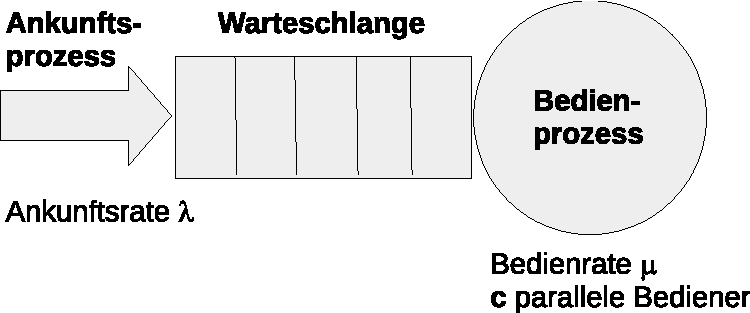
\includegraphics[width=0.6\textwidth]{ProofOfTheErlangCFormula-Modell.pdf}
\end{center}
\caption{Erlang-C-Warteschlangenmodell}
\label{fig:Model}
\end{figure}

Die langfristige Auslastung des Systems beträgt
$$
\rho:=\frac{\lambda}{c\mu}\;.
$$
Das System kann nur langfristig stabil arbeiten, wenn $\rho<1$ ist (die langfristige Ankunftsrate muss unterhalb der verfügbaren Bedienleistung liegen).


Üblicherweise interessiert man sich für die folgenden Kenngrößen des Systems:
\begin{itemize}
\item
$P(W\le t)$: Wahrscheinlichkeit dafür, dass ein neu eintreffender Kunde nicht länger als $t\ge0$ Sekunden warten muss (Erlang-C-Formel),
\item
$\mathbf{E}[W]$: mittlere Wartezeit,
\item
$\mathbf{E}[V]$: mittlere Verweilzeit,
\item
$\mathbf{E}[N_Q]$: mittlere Anzahl an Kunden in der Warteschlange,
\item
$\mathbf{E}[N]$: mittlere Anzahl an Kunden im System.
\end{itemize}



\section[Idee zur Herleitung von P(W<=t)]{Idee zur Herleitung von $P(W\le t)$}

Die Idee zur Berechnung der Wartezeitverteilung der Kunden $P(W\le t)$ (die Wahrscheinlichkeit, dass ein Kunde höchstens $t\ge0$ Sekunden warten muss) besteht darin, die Wartezeitverteilung für alle möglichen Zustände, in denen sich das System befinden kann, zu bestimmen und diese Zeiten mit der Wahrscheinlichkeit zu gewichten, dass sich das System im jeweiligen Zustand befindet. Dies führt zu folgender Formel:
\begin{equation}\label{eq:WaitingTimeDistribution1}
P(W\le t)=\sum_{n=0}^\infty P_{\mu,n-(c-1)}(W\le t)\cdot p_n\;,
\end{equation}
wobei $p_n$ die Wahrscheinlichkeit dafür ist, dass sich $n$ Kunden im System befinden, und $P_{\mu,m}(W\le t)$ die Wahrscheinlichkeit ist, dass ein neuer Kunde $t$ Sekunden oder weniger warten muss, wenn die Bedienrate $\mu>0$ ist und es $m$ Kunden gibt, die zunächst zu Ende bedient werden müssen, bevor der Bedienprozess für den neuen Kunden beginnt. Für $m=0$ beginnt der neue Bedienprozess sofort ($P_{\mu,0}(W\le t)=1$ für alle $t\ge0$) und aus Gründen der Konsistenz nehmen wir dasselbe für $m<0$ an.

\paragraph{Fall $n\ge c$:}~\\
Wenn sich $n<c$ Kunden im System befinden, kann ein neu eintreffender Kunde sofort bedient werden, da in diesem Fall nicht alle Bediener belegt sind. Wenn $n\ge c$ ist, müssen zunächst ein oder mehrere bereits laufende Bedienprozesse beendet werden, und dann müssen alle Kunden, die bereits vor dem neu angekommenen Kunden gewartet haben, bedient werden, bevor der neu angekommene Kunde bedient werden kann. Daher muss zwischen den Bediendauern von Kunden, deren Bedienprozess noch nicht begonnen hat, und den verbleibenden Bedienzeiten der Kunden, die sich bereits im Bedienprozess befinden, unterschieden werden. Da das Erlang-Modell jedoch die Exponentialverteilung für die Bedienzeiten verwendet, unterliegen diese beiden Zeitdauern derselben Wahrscheinlichkeitsverteilung mit demselben Parameter. Dies ist auf die Gedächtnislosigkeit der Exponentialverteilung zurückzuführen. (Diese Eigenschaft der Exponentialverteilung wird weiter unten in Abschnitt \ref{ExponentialDistribution} bewiesen).
\paragraph{Fall $n<c$:}~\\
Für $n<c$ Kunden im System ist die Wahrscheinlichkeit, dass ein neu eintreffender Kunde weniger als $t\ge0$ Sekunden warten muss, für alle $t\ge0$ immer 1 (da der neu eintreffende Kunde überhaupt nicht warten muss). Das bedeutet, dass $P_{\mu,n-(c-1)}(W\le t)=1$ für $n<c$ und für alle $t\ge0$ gilt und sich die Formel \eqref{eq:WaitingTimeDistribution1} vereinfacht zu:
\begin{equation}\label{eq:WaitingTimeDistribution2}
P(W\le t)=\sum_{n=0}^{c-1} p_n+\sum_{n=c}^\infty P_{\mu,n-(c-1)}(W\le t)\cdot p_n\;.
\end{equation}

Da $P_{\mu,n-(c-1)}(W\le t)$ die Hintereinandeausführung mehrerer Exponentialverteilungen bedeutet (und somit eine Erlang-Verteilung ist, siehe Abschnitt \ref{ErlangDistribution}) und $p_n$ die Wahrscheinlichkeit ist, dass sich die entsprechende Markov-Kette im Zustand $n$ befindet, werden in den folgenden Abschnitten Ergebnisse zu Exponentialverteilungen (Abschnitt \ref{ExponentialDistribution}), Erlang-Verteilungen (Abschnitt \ref{ErlangDistribution}) und Geburts- und Todesprozessen (Abschnitt \ref{BirthAndDeathProcesses}) vorgestellt. Auf Basis dieser Vorüberlegungen wird es dann möglich sein, die Erlang-C-Formel \eqref{eq:WaitingTimeDistribution2} in Abschnitt \ref{Result} zu berechnen.



\section{Exponentialverteilung}\label{ExponentialDistribution}

Da die Zwischenankunfts- und die Bedienzeiten in einem Erlang-Modell der Exponentialverteilung unterliegen, sollen im folgenden zunächst einige relevante Ergebnisse zu dieser Verteilung vorgestellt und bewiesen werden.

\begin{definition}[Dichte der Exponentialverteilung]
Die Funktion
$$
f_{\lambda}(x):=\left\{\begin{matrix}
\lambda \mathrm{e}^{-\lambda x},&~x\ge0\;,\\
0,&~x<0
\end{matrix}\right.
$$
mit $\lambda>0$ wird die Dichte der Exponentialverteilung genannt.
\end{definition}

\begin{theorem}[Verteilungsfunktion der Exponentialverteilung]
Die Funktion
$$
F_{\lambda}(x):=\left\{\begin{matrix}
1-\mathrm{e}^{-\lambda x},&~x\ge0\;,\\
0,&~x<0
\end{matrix}\right.
$$
ist die Verteilungsfunktion einer Exponentialverteilung mit Dichte $f_\lambda(x)$, $\lambda>0$.
\end{theorem}

\begin{proof}
Gemäß der Definition der Verteilungsfunktion $F(x):=\int_{-\infty}^x f(t)\,\mbox{d}t$ gilt:
$$
F_\lambda(x)=\int_0^x \lambda \mathrm{e}^{-\lambda t}\,\mbox{d}t=\left[-\mathrm{e}^{-\lambda t}\right]_{t=0}^{t=x}=-\mathrm{e}^{-\lambda x}-(-1)=1-\mathrm{e}^{-\lambda x}
$$
für $x\ge0$ und $F_\lambda(x)=0$ sonst.
\end{proof}

\begin{theorem}
Die Funktion $f_\lambda(x)$, $\lambda>0$, ist die Dichte einer Wahrscheinlichkeitsverteilung, d.\,h.\ es gelten $f_\lambda(x)\ge0$ und $\int_{-\infty}^\infty f_\lambda(x)\,\mbox{d}x=1$.
\end{theorem}

\begin{proof}
Die Behauptung $f_\lambda(x)\ge0$ ergibt sich unmittelbar aus der Definition von $f_\lambda(x)$. Mit dem vorherigen Satz gilt:
$$
\int_{-\infty}^\infty f_\lambda(t)\,\mbox{d}t=\lim_{x\to\infty}F_\lambda(x)=\lim_{x\to\infty}1-\mathrm{e}^{-\lambda x}=1\;.
$$
\end{proof}

\begin{theorem}[Kenngrößen der Exponentialverteilung]
Für eine Exponentialverteilung mit Parameter $\lambda>0$ gelten:
\begin{enumerate}
\item $\mathbf{E}[X]=\frac{1}{\lambda}$,
\item $\mathbf{Std}[X]=\frac{1}{\lambda}$ und
\item $\mathbf{CV}[X]=\mathbf{SCV}[X]=1$.
\end{enumerate}
\end{theorem}

\begin{proof}
\begin{enumerate}
\item
Mit der Definition von ${\mathbf E}[X]$ folgt:
\begin{eqnarray*}
{\mathbf E}[X]&=&
\int_{-\infty}^\infty x\cdot f_\lambda(x)\,\mbox{d}x=
\int_0^\infty \lambda x \mathrm{e}^{-\lambda x}\,\mbox{d}x\\&=&
\left[\lambda x\cdot\left(-\frac{1}{\lambda}\right)\mathrm{e}^{-\lambda x}\right]_{x=0}^{x=\infty}-
\int_0^\infty \lambda \left(-\frac{1}{\lambda}\right)\mathrm{e}^{-\lambda x}\,\mbox{d}x=
0+\int_0^\infty\mathrm{e}^{-\lambda x}\,\mbox{d}x\\&=&
\left[\left(-\frac{1}{\lambda}\right)\mathrm{e}^{-\lambda x}\right]_{x=0}^{x=\infty}=
0-\left(-\frac{1}{\lambda}\right)=
\frac{1}{\lambda}\;.
\end{eqnarray*}
\item
Mit der Definition von ${\mathbf E}[X^2]$ folgt zunächst:
\begin{eqnarray*}
{\mathbf E}[X^2]&=&
\int_{-\infty}^\infty x^2\cdot f_\lambda(x)\,\mbox{d}x=
\int_0^\infty \lambda x^2 \mathrm{e}^{-\lambda x}\,\mbox{d}x\\&=&
\left[\lambda x^2 \left(-\frac{1}{\lambda}\right)\mathrm{e}^{-\lambda x}\right]_{x=0}^{x=\infty}-
\int_0^\infty 2\lambda x \left(-\frac{1}{\lambda}\right)\mathrm{e}^{-\lambda x}\,\mbox{d}x=
0+\int_0^\infty 2x\mathrm{e}^{-\lambda x}\,\mbox{d}x\\&=&
\left[2x \left(-\frac{1}{\lambda}\right)\mathrm{e}^{-\lambda x}\right]_{x=0}^{x=\infty}-
\int_0^\infty 2\left(-\frac{1}{\lambda}\right)\mathrm{e}^{-\lambda x}\,\mbox{d}x=
0+\frac{2}{\lambda}\left[\left(-\frac{1}{\lambda}\right)\mathrm{e}^{-\lambda x}\right]_{x=0}^{x=\infty}\\&=&
0-\frac{2}{\lambda}\left(-\frac{1}{\lambda}\right)=
\frac{2}{\lambda^2}\;.
\end{eqnarray*}
Mit dem Verschiebungssatz gilt:
$$
\mathbf{Var}[X]={\mathbf E}[X^2]-\left({\mathbf E}[X]\right)^2=\frac{2}{\lambda^2}-\left(\frac{1}{\lambda}\right)^2=\frac{1}{\lambda^2}\;.
$$
Und damit gilt schließlich für die Standardabweichung:
$$
\mathbf{Std}[X]=\sqrt{\mathbf{Var}[X]}=\frac{1}{\lambda}\,.
$$
\item
Aus 1 und 2 folgt unmittelbar:
$$
\mathbf{CV}[X]=\frac{\mathbf{Std}[X]}{|{\mathbf E}[X]|}=\frac{\frac{1}{\lambda}}{\frac{1}{\lambda}}=1\,.
$$
Des Weiteren ist $\mathbf{SCV}[X]=\left(\mathbf{CV}[X]\right)^2=1$.
\end{enumerate}
\end{proof}

\subsection{Gedächtnislosigkeit der Exponentialverteilung}

\begin{theorem}[Gedächtnislosigkeit der Exponentialverteilung]
Ist eine Zeitdauer exponentiell verteilt und ist das Ereignis bis zum Zeitpunkt $s\ge0$ noch nicht eingetreten, so ist die Verteilungsfunktion der Wahrscheinlichkeitsverteilung, dass das Ereignis innerhalb der nächsten $t\ge0$ Zeiteinheiten eintritt (d.\,h.\ bis zu dem Zeitpunkt $s+t$), wieder exponentiell verteilt mit demselben Parameter $\lambda>0$, d.\,h.\ es gilt:
\begin{equation}\label{eq:DefinitionMemorylessness}
P(X\le t+s | X\ge s)=P(X\le t)\;,
\end{equation}
wobei $P(X\le a| X\ge b)$ die bedingte Wahrscheinlichkeit für das Ereignis "`$X\le a$"' unter dem Vorauswissen, dass $X\ge b$ ist, sei.
\end{theorem}

\begin{proof}
Mit den Rechenregeln für bedingte Wahrscheinlichkeiten gilt:
\begin{eqnarray*}
P(X\le t+s | X\ge s)&=&
\frac{P(\{X\le t+s\}\cap\{X\ge s\})}{P(X\ge s)}=
\frac{F_\lambda(t+s)-F_\lambda(s)}{1-F_\lambda(s)}\\&=&
\frac{1-\mathrm{e}^{-\lambda(t+s)}-1+\mathrm{e}^{-\lambda s}}{1-(1-\mathrm{e}^{-\lambda s})}=
\frac{\mathrm{e}^{-\lambda s}-\mathrm{e}^{-\lambda(t+s)}}{\mathrm{e}^{-\lambda s}}=
1-\mathrm{e}^{-\lambda t}\\&=&
F_\lambda(t)=
P(X\le t)\;.
\end{eqnarray*}
\end{proof}

\paragraph{Konsequenz:}~\\
Ist die Bediendauer eines Kunden exponentiell verteilt mit Parameter $\lambda>0$ und befindet sich der Kunde bereits in Bedienung, so ist seine Restbediendauer wiederum exponentiell verteilt mit demselben Parameter $\lambda$. Soll die Verteilungsfunktion der Wartezeit eines neu eintreffenden Kunden bestimmt werden, so muss also nicht zwischen den Restbedienzeiten der momentan in Bedienung befindlichen Kunden und den Bedienzeiten der vor dem neu eingetroffenen Kunden wartenden anderen Kunden unterschieden werden.

\begin{theorem}
Die Exponentialverteilung $F_\lambda(x)$ ist die einzige \emph{stetige} Verteilungsfunktion mit $F(x)=0$ für $x\le0$, die die Eigenschaft der
\end{theorem}

\begin{proof}
Der Beweis erfolgt in drei Schritten:

\paragraph{Schritt 1: Funktionalgleichung zur Beschreibung der Gedächtnislosigkeit}~\\
Um den Beweis formal möglichst einfach darstellen zu können, wird zunächst die Funktion $G(t):=1-F(t)$ definiert, die die Wahrscheinlichkeit angibt, dass das Ereignis bis zum Zeitpunkt $t\ge0$ \emph{noch nicht} eingetreten ist. (Diese Definition stammt aus der Zuverlässigkeitstheorie; dort wird $G(t)$ auch die \emph{Überlebenswahrscheinlichkeit}\index{Ueberlebenswahrscheinlichkeit@Überlebenswahrscheinlichkeit} genannt.) Aus Gleichung \eqref{eq:DefinitionMemorylessness} wird damit mit Hilfe der Rechenregeln für bedingte Wahrscheinlichkeiten:
\begin{eqnarray*}
~&~&P(X\le t+s | X\ge s)=P(X\le t)
~\iff~\frac{F(t+s)-F(s)}{1-F(s)}=F(t)\\
~&\iff&\frac{1-G(t+s)-(1-G(s))}{G(s)}=1-G(t)\\
~&\iff&-G(t+s)+G(s)=G(s)-G(s)G(t)
~\iff~G(s+t)=G(s)G(t)\,.
\end{eqnarray*}
Es ist jetzt also zu zeigen, dass nur die Überlebenswahrscheinlichkeit unter Annahme einer Exponentialverteilung, d.\,h.\ $G_\lambda(t)=\mathrm{e}^{-\lambda t}$, die Gleichung $G(s+t)=G(s)G(t)$ erfüllt.

\paragraph{Schritt 2: Explizite Darstellung für $G(t)$}~\\
Aus $G(s+t)=G(s)G(t)$ folgt für $a\in\mathbb{N}$ und $b\in\mathbb{N}$:
\begin{eqnarray*}
G\left(\frac{a}{b}\right)&=&
G\left(\frac{1}{b}+\frac{a-1}{b}\right)=
G\left(\frac{1}{b}\right)\cdot G\left(\frac{a-1}{b}\right)=
\ldots=
\underbrace{G\left(\frac{1}{b}\right)\cdots G\left(\frac{1}{b}\right)}_{a~\textrm{Faktoren}}\\
&=&\left[G\left(\frac{1}{b}\right)\right]^a\,.
\end{eqnarray*}
Mit $1=\frac{b}{b}$ gilt außerdem $G(1)=\left[G\left(\frac{1}{b}\right)\right]^b$ bzw.\ $\left[G(1)\right]^{\frac{1}{b}}=G\left(\frac{1}{b}\right)$.
Damit folgt weiter:
$$
G\left(\frac{a}{b}\right)=
\left[G\left(\frac{1}{b}\right)\right]^a=
\left[G(1)\right]^{\frac{a}{b}}\,.
$$
Das bedeutet, dass der Zusammenhang $G(q)=[G(1)]^q$ für alle positiven, rationalen Zahlen $q$ gilt. Aufgrund der Tatsache, dass $F$ als stetig angenommen wurde und somit auch $G$ stetig ist, gilt $G(t)=[G(1)]^t$ für alle reellen $t\ge0$. Weiter gilt mit den Rechenregeln für die Exponentialfunktion und Logarithmen:
$$
G(t)=
\mathrm{e}^{\ln\left(G(1)^t\right)}=
\mathrm{e}^{t\ln(G(1))}\,.
$$
Mit der Wahl von $\lambda:=-\ln(G(1))$ folgt $G(t)=\mathrm{e}^{-\lambda t}$ bzw.\ $F(t)=1-\mathrm{e}^{-\lambda t}$.
Zu zeigen bleibt, dass $0<\lambda<\infty$ bzw.\ $0<G(1)<1$ gilt.

\paragraph{Schritt 3: Nachweis, dass $0<G(1)<1$ gilt}~\\
Es ist $G(1)=1-F(1)$. Damit gilt sofort $0\le G(1)\le1$. Zu zeigen bleibt $0\neq G(1)\neq1$.
\begin{itemize}
\item
Wenn $G(1)=0$ wäre, würde $G(x)=\left[G(1)\right]^x=0^x=0$ für alle $x>0$ gelten. Damit wäre $F(x)=1$ für alle $x>0$. Da aber $F$ als stetig vorausgesetzt wurde und außerdem $F(0)=0$ nach Voraussetzung galt, kann dies nicht der Fall sein.
\item
Wenn $G(1)=1$ wäre, würde $G(x)=\left[G(1)\right]^x=1^x=1$ für alle $x\ge0$ gelten. Damit wäre $F(x)=0$ für alle $x\ge0$, was im Widerspruch dazu steht, dass $F(x)$ die Verteilungsfunktion einer Wahrscheinlichkeitsverteilung ist und somit $\lim_{x\to\infty}F(x)=1$ gelten muss.
\end{itemize}
\end{proof}



\section{Faltung von Wahrscheinlichkeitsverteilungen}

Werden zwei Prozesse, die durch Wahrscheinlichkeitsverteilungen beschrieben werden können, hintereinander ausgeführt, so spricht man davon, dass die Dichten der beiden Wahrscheinlichkeitsverteilungen miteinander gefaltet werden. Das Ergebnis der Faltung ist die Dichte der Wahrscheinlichkeitsverteilung, die den Gesamtprozess beschreibt.

\begin{definition}[Faltung]
Sind $f(x)$ und $g(x)$ die Dichten von zwei Wahrscheinlichkeitsverteilungen, so nennt man
$$
f*g(x):=\int_{-\infty}^\infty f(t)g(x-t)\,\mbox{d}t
$$
die Faltung von $f$ und $g$.
\end{definition}

Anschaulich werden durch obige Formel alle denkbaren Fälle, wie die Gesamtzeit $x$ auf die beiden Teilprozesse $f$ und $g$ aufgeteilt werden kann, aufintegriert.

Da die Faltung durch ein Integral über das Produkt von zwei Dichten definiert ist, gilt auch hier wieder, dass diese für alle Wahrscheinlichkeitsverteilungen, bei denen die Bestimmung der Stammfunktion der Dichte schwierig ist -- was für fast alle stetigen Wahrscheinlichkeitsverteilungen außer der Exponentialverteilung gilt --, nur sehr schwierig oder überhaupt nicht explizit berechenbar ist. Daher wird in den Erlang-Formeln grundsätzlich die Exponentialverteilung für die Bedienzeiten verwendet.



\section{Erlang-Verteilung}\label{ErlangDistribution}

Wie sich im Folgenden zeigen wird, beschreibt die Erlang-Verteilung einen Prozess, der aus der Hintereinanderausführung von $n\in\mathbb{N}$ Teilprozessen besteht, deren Zeitdauern jeweils mit demselben Parameter $\lambda>0$ exponentiell verteilt sind.

In einem M/M/1-System lässt sich die Wartezeitverteilung eines neu eintreffenden Kunden durch die Bediendauern der vor ihm wartenden Kunden und der Restbediendauer des gerade in Bedienung befindlichen Kunden darstellen. Aufgrund der Gedächtnislosigkeit der Exponentialverteilung ist die Restbediendauer des momentan in Bedienung befindlichen Kunden aber genauso verteilt, wie seine gesamte Bediendauer (siehe Gleichung \eqref{eq:DefinitionMemorylessness}). D.\,h.\ befinden sich vor dem neu eintreffenden Kunden bereits $k\ge0$ Kunden in der Warteschlange und sind die Bediendauern mit Parameter $\mu\ge0$ exponentiell verteilt, so ist die Wartezeit des neuen Kunden Erlang-verteilt mit den Parametern $\mu$ und $k+1$.

\begin{definition}[Dichte der Erlang-Verteilung]
Die Funktion
$$
f_{\lambda,n}(x):=\left\{\begin{matrix}
\frac{\lambda^n x^{n-1}}{(n-1)!} \mathrm{e}^{-\lambda x},&~x\ge0\;,\\
0,&~x<0
\end{matrix}\right.
$$
mit $\lambda>0$ und $n\in\mathbb{N}$ wird die Dichte der Erlang-Verteilung genannt.
\end{definition}

\begin{theorem}[Zusammenhang mit der Exponentialverteilung]
Die Funktion $f_{\lambda,n}(x)$, $\lambda>0$, $n\in\mathbb{N}$ ist die $n$-fache Faltung von $f_\lambda(x)$.
\end{theorem}

\begin{proof}
Der Beweis wird per Induktion geführt. Offensichtlich gilt $f_{\lambda,1}(x)=\lambda \mathrm{e}^{-\lambda x}=f_\lambda(x)$. Für die Faltung von zwei exponentiell verteilten Zeitdauern gilt:
$$
f_{\lambda,1}*f_\lambda(x)=
f_\lambda*f_\lambda(x)=
\int_0^x \lambda \mathrm{e}^{-\lambda t}\cdot\lambda \mathrm{e}^{-\lambda(x-t)}\,\mbox{d}t=
\left[\lambda^2\mathrm{e}^{-\lambda x}t\right]_{t=0}^{t=x}=
\lambda^2x\mathrm{e}^{-\lambda x}=f_{\lambda,2}(x)
$$
für $x\ge0$ und $f_{\lambda,2}(x)=0$ sonst. Es wird nun angenommen, dass
$$
f_{\lambda,n}(x)=\underbrace{f_\lambda*\cdots*f_\lambda}_{n~{\rm-fach}}(x)
$$
für ein $n\in\mathbb{N}$ gelte.
Dann gilt:
\begin{eqnarray*}
f_{\lambda,n}*f_\lambda(x)&=&
\int_0^x \frac{\lambda^n t^{n-1}}{(n-1)!}\mathrm{e}^{-\lambda t}\cdot\lambda \mathrm{e}^{-\lambda(x-t)}\,\mbox{d}t=
\frac{\lambda^{n+1}}{(n-1)!}\mathrm{e}^{-\lambda x}\int_0^x t^{n-1}\,\mbox{d}t\\&=&
\frac{\lambda^{n+1}}{(n-1)!}\mathrm{e}^{-\lambda x}\left[\frac{1}{n}t^n\right]_{t=0}^{t=x}=
\frac{\lambda^{n+1}x^n}{n!}\mathrm{e}^{-\lambda x}=
f_{\lambda,n+1}(x)
\end{eqnarray*}
für $x\ge0$ und $f_{\lambda,n+1}(x)=0$ sonst.
\end{proof}

\begin{theorem}[Verteilungsfunktion der Erlang-Verteilung]
Die Funktion
$$
F_{\lambda,n}(x):=\left\{\begin{matrix}
1-\mathrm{e}^{-\lambda x}\sum_{i=0}^{n-1}\frac{(\lambda x)^i}{i!},&~x\ge0\;,\\
0,&~x<0
\end{matrix}\right.
$$
ist die Verteilungsfunktion einer Erlang-Verteilung mit Dichte $f_{\lambda,n}(x)$, $\lambda>0$, $n\in\mathbb{N}$.
\end{theorem}

\begin{proof}
Der Beweis wird ebenfalls per Induktion geführt. Für den Fall $n=1$ gilt:
$$
F_{\lambda,1}(x)=1-\mathrm{e}^{-\lambda x}\underbrace{\sum_{i=0}^{1-1}\frac{(\lambda x)^i}{i!}}_{=1}=F_{\lambda}(x)\;.
$$
Da $F_{\lambda}(x)$ die Verteilungsfunktion der Exponentialverteilung ist und $f_{\lambda,1}(x)=f_\lambda(x)$ galt, ist damit der Induktionsanfang gezeigt. Es wird nun angenommen, dass bereits bekannt sei, dass
$$
F_{\lambda,n-1}(x)=1-\mathrm{e}^{-\lambda x}\sum_{i=0}^{n-2}\frac{(\lambda x)^i}{i!}
$$
für ein $n\in\mathbb{N}$, $n\ge2$, für $x\ge0$ gelte. Dann ist:
\begin{eqnarray*}
F_{\lambda,n}(x)&=&
\int_0^x f_{\lambda,n}(t)\,\mbox{d}t=
\int_0^x \frac{\lambda^n t^{n-1}}{(n-1)!}\mathrm{e}^{-\lambda t}\,\mbox{d}t\\&=&
\left[\frac{\lambda^n t^{n-1}}{(n-1)!}\left(-\frac{1}{\lambda}\mathrm{e}^{-\lambda t}\right)\right]_{t=0}^{t=x}-\int_0^x\frac{\lambda^n t^{n-2}}{(n-2)!}\left(-\frac{1}{\lambda}\mathrm{e}^{-\lambda t}\right)\,\mbox{d}t\\&=&
-\frac{(\lambda x)^{n-1}}{(n-1)!}\mathrm{e}^{-\lambda x}+\int_0^x f_{\lambda,n-1}(t)\,\mbox{d}t=
-\frac{(\lambda x)^{n-1}}{(n-1)!}\mathrm{e}^{-\lambda x}+F_{\lambda,n-1}(t)\\&=&
-\frac{(\lambda x)^{n-1}}{(n-1)!}\mathrm{e}^{-\lambda x}+1-\mathrm{e}^{-\lambda x}\sum_{i=0}^{n-2}\frac{(\lambda x)^i}{i!}=
1-\mathrm{e}^{-\lambda x}\sum_{i=0}^{n-1}\frac{(\lambda x)^i}{i!}
\end{eqnarray*}
für $x\ge0$ und $F_{\lambda,n}(x)=0$ sonst.
\end{proof}

\begin{theorem}
Die Funktion $f_{\lambda,n}(x)$, $\lambda>0$, $n\in\mathbb{N}$, ist die Dichte einer Wahrscheinlichkeitsverteilung, d.\,h.\ es gelten $f_{\lambda,n}(x)\ge0$ und
$$
\int_{-\infty}^\infty f_{\lambda,n}(x)\,\mbox{d}x=1\;.
$$
\end{theorem}

\begin{proof}
Die Behauptung $f_{\lambda,n}(x)\ge0$ ergibt sich unmittelbar aus der Definition von $f_{\lambda,n}(x)$. Mit der Reihendarstellung der Exponentialfunktion liefert die $n$-fache Anwendung der Regel von l'Hospital:
$$
F_{\lambda,n}(x)=
1-\mathrm{e}^{-\lambda x}\sum_{i=0}^{n-1}\frac{(\lambda x)^i}{i!}=
1-\frac{\sum_{i=0}^{n-1}\frac{(\lambda x)^i}{i!}}{\sum_{i=0}^{\infty}\frac{(\lambda x)^i}{i!}}
\mathop{\longrightarrow}\limits^{x\to\infty}1\;.
$$
Damit gilt:
$$
\int_{-\infty}^\infty f_{\lambda,n}(t)\,\mbox{d}t=
\lim_{x\to\infty}F_{\lambda,n}(x)=1\;.
$$
\end{proof}

\begin{theorem}[Kenngrößen der Erlang-Verteilung]
Für eine Erlang-Verteilung mit Parametern $\lambda>0$ und $n\in\mathbb{N}$ gelten:
\begin{enumerate}
\item $\mathbf{E}[X]=\frac{n}{\lambda}$,
\item $\mathbf{Std}[X]=\frac{\sqrt{n}}{\lambda}$ und
\item $\mathbf{CV}[X]=\frac{1}{\sqrt{n}}$ and $\mathbf{SCV}[X]=\frac{1}{n}$.
\end{enumerate}
\end{theorem}

\begin{proof}
Die Erlang-Verteilung mit den Parametern $\lambda>0$ und $n\in\mathbb{N}$ stellt die Hintereinanderausführung von $n$ unabhängigen Exponentialverteilungen mit Parameter $\lambda$ dar. Aufgrund der Unabhängigkeit der einzelnen Teilprozesse dürfen nicht nur die Erwartungswerte addiert werden, sondern auch die Varianzen. Für den Erwartungswert der Erlang-Verteilung folgt damit sofort
$$
{\mathbf E}[X]=n\cdot\frac{1}{\lambda}=\frac{n}{\lambda}\;.
$$
Für die Standardabweichung gilt:
$$
\mathbf{Std}[X]=\sqrt{\mathbf{Var}[X]}=\sqrt{n\cdot\frac{1}{\lambda^2}}=\frac{\sqrt{n}}{\lambda}\,.
$$
Damit gilt unmittelbar für den Variationskoeffizienten:
$$
\mathbf{CV}[X]=\frac{\mathbf{Std}[X]}{|{\mathbf E}[X]|}=\frac{\frac{\sqrt{n}}{\lambda}}{\frac{n}{\lambda}}=\frac{1}{\sqrt{n}}\,.
$$
Des Weiteren ist damit $\mathbf{SCV}[X]=\left(\mathbf{CV}[X]\right)^2=\frac{1}{n}$.
\end{proof}



\section{Geburts- und Todesprozesse}\label{BirthAndDeathProcesses}

Markov-Prozesse, bei denen nur Übergänge zu dem jeweils nächst höheren Zustand oder dem nächst niedrigeren Zustand möglich sind (z.\,B.\ Ankünfte und Abgänge von einzelnen Kunden), werden Geburts- und Todesprozesse genannt. Eine ,,Geburt'' stellt die Ankunft eines Kunden dar, ein ,,Tod'' den Abgang eines zu Ende bedienten Kunden, siehe Abbildung \ref{fig:BirthAndDEathProcess}.

\begin{figure}[H]
\begin{center}
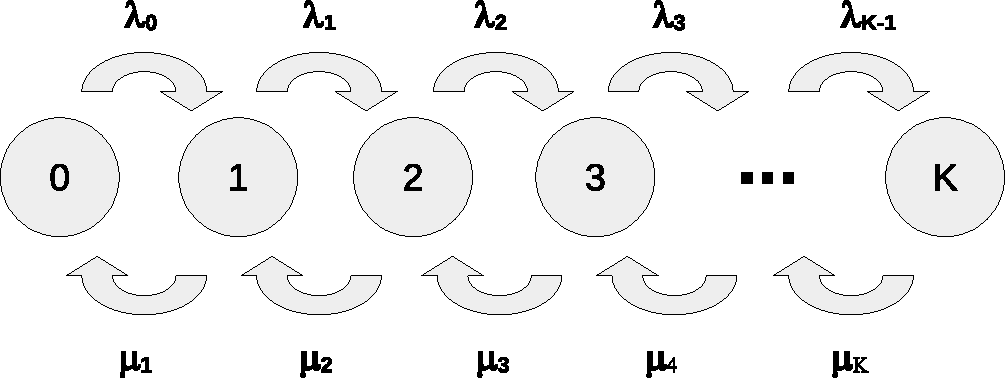
\includegraphics[width=0.6\textwidth]{ProofOfTheErlangCFormula-MarkovChain.pdf}
\end{center}
\caption{Ein Geburts- und Todesprozess dargestellt als Markov-Kette}
\label{fig:BirthAndDEathProcess}
\end{figure}

\subsection{Ankunfts- und Bedienrate}

Für die zustandsabhängige Ankunftsrate am System in einem Bedienprozess mit $K\in\mathbb{N}$ Warte- und Bedienplätzen gilt für den Zustand $n\in\mathbb{N}_0$:
\begin{equation}\label{GleichungMarkovAnkunftsrate}
\lambda_n^{\rm Sys}:=\left\{\begin{matrix}
\lambda,&~n<K\;,\\
0,&~n=K\;,
\end{matrix}\right.
\end{equation}
wobei $\lambda>0$ die Ankunftsrate bezogen auf die Kunden ist. Befinden sich bereits $n=K$ Kunden im System, so können keine weiteren Kunden am System eintreffen, d.\,h.\ es ist in diesem Fall $\lambda^{\rm Sys}=0$.

Für die zustandsabhängige Bedienrate bezogen auf das gesamte System gilt:
\begin{equation}\label{GleichungMarkovBedienrate}
\mu_n^{\rm Sys}:=\left\{\begin{matrix}
n\mu,&~n\le c\;,\\
c\mu,&~n>c\;,
\end{matrix}\right.
\end{equation}
wobei $\mu>0$ die Bedienrate eines einzelnen Bedieners ist.

\subsection{Transiente Zustandswahrscheinlichkeiten}

Es wird nun angenommen, dass die Wahrscheinlichkeit $p_n(t)$, mit der sich zu einem Zeitpunkt $t\ge0$ insgesamt $n\in\mathbb{N}_0$ Kunden im System befinden, zu einem bestimmten vorgegebenen Zeitpunkt $t\ge0$ bekannt sei. Auf dieser Basis wird bestimmt, mit welcher Wahrscheinlichkeit zu einem Zeitpunkt $t+\Delta t$ sich $n\in\mathbb{N}_0$ Kunden im System befinden. Dabei kann man sich $\Delta t>0$ als einen kleinen Augenblick vorstellen, der seit dem Zeitpunkt $t$ vergangen ist. Im Fall $n=0$ setzt sich $p_0(t+\Delta t)$ aus der Wahrscheinlichkeit, dass zum Zeitpunkt $t$ auch bereits 0 Personen im System waren und kein Kunde eingetroffen ist, und der Wahrscheinlichkeit, dass zum Zeitpunkt $t$ ein Kunde im System war und dieser in der Zeit $\Delta t$ zu Ende bedient wurde, zusammen. Des Weiteren könnten in der Zeitdauer $\Delta t$ auch ein Kunde eingetroffen und bereits wieder aus dem System ausgeschieden sein usw.\ Im Vergleich zu den zuerst genannten beiden Wahrscheinlichkeiten sind die Wahrscheinlichkeiten für solche Ereignisse jedoch verschwindend gering -- mathematisch spricht man davon, dass sie für $\Delta t\to0$ schneller gegen 0 konvergieren als $\Delta t$. Dies drückt man durch das Landau-Symbol $o(\Delta t)$ aus. Damit ergibt sich für $n=0$:
$$
p_0(t+\Delta t)=
p_0(t)(1-\Delta t\lambda_0^{\rm Sys})+p_1(t)\Delta t\mu_1^{\rm Sys}+o(\Delta t)\;.
$$
Für $n=1,\ldots,K-1$ ergibt sich zusätzlich die Möglichkeit, dass der Zustand $n$ aus dem Zustand $n-1$ heraus erreicht wurde:
$$
p_n(t+\Delta t)=
p_n(t)(1-\Delta t\lambda_n^{\rm Sys}-\Delta t\mu_n^{\rm Sys})+p_{n-1}(t)\Delta t\lambda_{n-1}^{\rm Sys}+p_{n+1}(t)\Delta t\mu_{n+1}^{\rm Sys}+o(\Delta t)\;.
$$
Für $n=K$ schließlich kann der Zustand nur aus den Vorgängerzuständen $n$ und $n-1$ heraus erreicht werden:
$$
p_K(t+\Delta t)=
p_K(t)(1-\Delta t\mu_K^{\rm Sys})+p_{K-1}(t)\Delta t\lambda_{K-1}^{\rm Sys}+o(\Delta t)\;.
$$

\subsection{Stationäre Zustandswahrscheinlichkeiten}

Termumformung in den drei obigen Gleichungen ergibt zunächst (für $n=1,\ldots,K-1$ in der mittleren Gleichung):
\begin{eqnarray}
\frac{p_0(t+\Delta t)-p_0(t)}{\Delta t}&=&
-p_0(t)\lambda_0^{\rm Sys}+p_{1}(t)\mu_1^{\rm Sys}+\frac{o(\Delta t)}{\Delta t}\;,
\label{eq:StationaryStateProbabilities1}\\
\frac{p_n(t+\Delta t)-p_n(t)}{\Delta t}&=&
-p_n(t)(\lambda_n^{\rm Sys}+\mu_n^{\rm Sys})+p_{n+1}(t)\mu_{n+1}^{\rm Sys}+p_{n-1}(t)\lambda_{n-1}^{\rm Sys}+\frac{o(\Delta t)}{\Delta t}\;,
\nonumber\\
\frac{p_K(t+\Delta t)-p_K(t)}{\Delta t}&=&
-p_K(t)\mu_K^{\rm Sys}+p_{K-1}(t)\lambda_{K-1}^{\rm Sys}+\frac{o(\Delta t)}{\Delta t}\;.
\nonumber
\end{eqnarray}
Wählt man nun für $\Delta t$ eine immer kürzere Zeitspanne, d.\,h.\ führt man den Grenzübergang $\Delta t\to0$ durch, so ergibt sich für $n=0,\ldots,K$
auf den linken Seiten der Gleichungen \eqref{eq:StationaryStateProbabilities1}:
$$
\lim_{\Delta t\to0}\frac{p_n(t+\Delta t)-p_n(t)}{\Delta t}=p'_n(t)\;.
$$
Des Weiteren gilt $\lim_{\Delta t\to0}\frac{o(\Delta t)}{\Delta t}=0$ nach Definition von $o(\Delta t)$. Damit wird für $\Delta t\to0$ aus \eqref{eq:StationaryStateProbabilities1}:
\begin{eqnarray}
p'_0(t)&=&
-p_0(t)\lambda_0^{\rm Sys}+p_{1}(t)\mu_1^{\rm Sys}\;,
\nonumber\\
p'_n(t)&=&
-p_n(t)(\lambda_n^{\rm Sys}+\mu_n^{\rm Sys})+p_{n+1}(t)\mu_{n+1}^{\rm Sys}+p_{n-1}(t)\lambda_{n-1}^{\rm Sys}\;,
\label{eq:StationaryStateProbabilities2}\\
p'_K(t)&=&
-p_K(t)\mu_K^{\rm Sys}+p_{K-1}(t)\lambda_{K-1}^{\rm Sys}\;.
\nonumber
\end{eqnarray}
Die Betrachtung eines Warteschlangensystems im stationären Zustand bedeutet, dass man das System nach sehr langer Laufzeit, also für $t\to\infty$ betrachtet. Der stationäre Zustand zeichnet sich in einem System, welches diesen erreicht, also in dem z.\,B.\ nicht kontinuierlich mehr Kunden eintreffen, als bedient werden können, dadurch aus, dass sich die Zustandswahrscheinlichkeiten stabilisieren, d.\,h.\ es gilt $p'_n(t)\to0$ für alle $n=0,\ldots,K$ für $t\to\infty$.
Setzt man in \eqref{eq:StationaryStateProbabilities2}	$p'_n(t)=0$ so ergibt sich das folgende lineare Gleichungssystem für die stationären, d.\,h.\ zeitunabhängigen, Zustandswahrscheinlichkeiten $p_n:=\lim_{t\to\infty}p_n(t)$:
\begin{eqnarray}
p_1&=&
\frac{\lambda_0^{\rm Sys}}{\mu_1^{\rm Sys}}p_0\;,
\nonumber\\
p_{n+1}&=&
\frac{\lambda_n^{\rm Sys}}{\mu_{n+1}^{\rm Sys}}p_n+\frac{\mu_n^{\rm Sys}}{\mu_{n+1}^{\rm Sys}}p_n-\frac{\lambda_{n-1}^{\rm Sys}}{\mu_{n+1}^{\rm Sys}}p_{n-1}\;,
\label{eq:StationaryStateProbabilities3}\\
p_K&=&
\frac{\lambda_{K-1}^{\rm Sys}}{\mu_K^{\rm Sys}}p_{K-1}\;.
\nonumber
\end{eqnarray}

\begin{theorem}
Mit den obigen Bezeichnungen gelten:
\begin{equation}
p_n=\prod_{i=1}^n\frac{\lambda_{i-1}^{\rm Sys}}{\mu_i^{\rm Sys}}p_0 ~~~\textrm{für}~ n=1,\ldots,K
~~~\textrm{und}~~~
p_0=\left[\sum_{n=1}^K\prod_{i=1}^n\frac{\lambda_{i-1}^{\rm Sys}}{\mu_i^{\rm Sys}}+1\right]^{-1}\;.
\label{eq:StationaryStateProbabilities4}
\end{equation}
\end{theorem}

\begin{proof}
Der Beweis für $p_n$, $n=1,\ldots,K$, erfolgt per Induktion. Der Induktionsanfang ergibt sich unmittelbar aus der ersten Gleichung von \eqref{eq:StationaryStateProbabilities3}. Es sei nun angenommen, dass die Gleichung \eqref{eq:StationaryStateProbabilities4} für ein $n\in\mathbb{N}$ gelte. Dann ergibt sich aus der zweiten Gleichung von \eqref{eq:StationaryStateProbabilities3} für $n+1$:
\begin{eqnarray*}
p_{n+1}&=&
\frac{\lambda_n^{\rm Sys}}{\mu_{n+1}^{\rm Sys}}p_n+\frac{\mu_n^{\rm Sys}}{\mu_{n+1}^{\rm Sys}}p_n-\frac{\lambda_{n-1}^{\rm Sys}}{\mu_{n+1}^{\rm Sys}}p_{n-1}\\&=&
\frac{\lambda_n^{\rm Sys}}{\mu_{n+1}^{\rm Sys}}\prod_{i=1}^n\frac{\lambda_{i-1}^{\rm Sys}}{\mu_i^{\rm Sys}}p_0+
\frac{\mu_n^{\rm Sys}}{\mu_{n+1}^{\rm Sys}}\prod_{i=1}^n\frac{\lambda_{i-1}^{\rm Sys}}{\mu_i^{\rm Sys}}p_0-
\frac{\lambda_{n-1}^{\rm Sys}}{\mu_{n+1}^{\rm Sys}}\prod_{i=1}^{n-1}\frac{\lambda_{i-1}^{\rm Sys}}{\mu_i^{\rm Sys}}p_0\\&=&
\prod_{i=1}^{n+1}\frac{\lambda_{i-1}^{\rm Sys}}{\mu_i^{\rm Sys}}p_0+
\underbrace{\left[\frac{\mu_n^{\rm Sys}\lambda_{n-1}^{\rm Sys}}{\mu_{n+1}^{\rm Sys}\mu_n^{\rm Sys}}-\frac{\lambda_{n-1}^{\rm Sys}}{\mu_{n+1}^{\rm Sys}}\right]}_{=0}
\prod_{i=1}^{n-1}\frac{\lambda_{i-1}^{\rm Sys}}{\mu_i^{\rm Sys}}p_0\;.
\end{eqnarray*}
Das Warteschlangensystem muss sich stets in einem der Zustände $0,\ldots,K$ befinden, d.\,h.\ die Summe aller Wahrscheinlichkeiten muss 1 ergeben ($\sum_{n=0}^Kp_n=1$). Mit der Formel $p_n$ ergibt sich:
$$
p_0+\sum_{n=1}^K\prod_{i=1}^n\frac{\lambda_{i-1}^{\rm Sys}}{\mu_i^{\rm Sys}}p_0=1\;.
$$
Löst man diese Gleichung nach $p_0$ auf, so ergibt sich sofort die Aussage für $p_0$.
\end{proof}

\subsection{Stationäre Zustandswahrscheinlichkeiten für die konkreten Ankunfts- und Bedienraten}

Bisher wurden in den Formeln für die Zustandswahrscheinlichkeiten die Ankunftsrate bezogen auf das Gesamtsystem $\lambda^{\rm Sys}$ und die Bedienrate des Gesamtsystems $\mu^{\rm Sys}$ verwendet. Im Folgenden sollen nun die Ankunftsraten der einzelnen Kunden $\lambda$ bzw.\ die Bedienraten der einzelnen Bedieners $\mu$ verwendet werden. Die Größen $\lambda^{\rm Sys}$ und $\mu^{\rm Sys}$ sind für drei Bereiche unterschiedlich definiert: für $n=0$, für $n=1,\ldots,c$ und für $n=c+1,\ldots,K$. Aus diesem Grund wird $p_n$ im Folgenden auch für diese Bereiche getrennt berechnet:

\subsubsection*{Bestimmung von $p_0$}

Setzt man die Zustandswahrscheinlichkeiten aus \eqref{GleichungMarkovAnkunftsrate} und \eqref{GleichungMarkovBedienrate} für $p_0$ in \eqref{eq:StationaryStateProbabilities4} ein, so ergibt sich:
\begin{eqnarray*}
p_0&=&
\left[\sum_{n=1}^K\prod_{i=1}^n\frac{\lambda_{i-1}^{\rm Sys}}{\mu_i^{\rm Sys}}+1\right]^{-1} =
\left[\sum_{n=1}^K\left(
\lambda^n\cdot\frac{1}{\prod_{i=1}^{\min(n,c)}i\mu\cdot\prod_{i=\min(n,c)+1}^nc\mu}
\right)+1\right]^{-1}\\&=&
\left[\sum_{n=1}^c\frac{\lambda^n}{\mu^nn!}+\sum_{n=c+1}^K\frac{\lambda^n}{\mu^cc!\cdot(c\mu^{n-c})}+1\right]^{-1} =
\left[\sum_{n=1}^c\frac{\lambda^n}{\mu^nn!}+\sum_{n=c+1}^K\frac{\lambda^n}{\mu^nc!c^{n-c}}+1\right]^{-1}\;.
\end{eqnarray*}
Mit $a:=\frac{\lambda}{\mu}$ gilt weiter:
$$
p_0=
\left[\sum_{n=1}^c\frac{a^n}{n!}+\sum_{n=c+1}^K\frac{a^n}{c!c^{n-c}}+1\right]^{-1}\;.
$$
Mit der Wahl von
\begin{equation}\label{MathematikErlangCn}
C_n:=\left\{\begin{array}{ll}
\displaystyle \frac{a^n}{n!}&~~\textrm{für}~n\le c\;,\\
\displaystyle \frac{a^n}{c!c^{n-c}}&~~\textrm{für}~c<n\le K
\end{array}\right.
\end{equation}
gilt schließlich
$$
p_0=\left[\sum_{n=0}^KC_n\right]^{-1}\;.
$$

\subsubsection*{Bestimmung von $p_n$ für $n=1,\ldots,c$}

Setzt man die Zustandswahrscheinlichkeiten aus \eqref{GleichungMarkovAnkunftsrate} und \eqref{GleichungMarkovBedienrate} für $p_n$ in \eqref{eq:StationaryStateProbabilities4} ein, so ergibt sich mit der Definition von $C_n$ in \eqref{MathematikErlangCn} für $n=1,\ldots,c$:
$$
p_n=
\prod_{i=1}^n\frac{\lambda_{i-1}^{\rm Sys}}{\mu_i^{\rm Sys}}\cdot p_0=
\prod_{i=1}^n\frac{\lambda}{n\mu}\cdot p_0=
\frac{a^n}{n!}\cdot p_0=
C_np_0\;.
$$

\subsubsection*{Bestimmung von $p_n$ für $n=c+1,\ldots,K$}

Setzt man die Zustandswahrscheinlichkeiten aus \eqref{GleichungMarkovAnkunftsrate} und \eqref{GleichungMarkovBedienrate} für $p_n$ in \eqref{eq:StationaryStateProbabilities4} ein, so ergibt sich mit der Definition von $C_n$ in \eqref{MathematikErlangCn} für $n=c+1,\ldots,K$:
\begin{eqnarray*}
p_n&=&
\prod_{i=1}^n\frac{\lambda_{i-1}^{\rm Sys}}{\mu_i^{\rm Sys}}\cdot p_0=
\prod_{i=1}^c\frac{\lambda}{n\mu}\cdot\prod_{i=c+1}^n\frac{\lambda}{c\mu}\cdot p_0=
\frac{a^n}{c!c^{n-c}}\cdot p_0=
C_np_0\;.
\end{eqnarray*}

Die obigen Überlegungen für $p_n$ lassen sich zu folgendem Satz zusammenfassen:

\begin{theorem}
Mit der Wahl von $C_n$ gemäß \eqref{MathematikErlangCn} gilt für die Zustandswahrscheinlichkeiten $p_n$ in einem Geburts- und Todesprozess mit Ankunfts- und Bedienraten gemäß \eqref{GleichungMarkovAnkunftsrate} und \eqref{GleichungMarkovBedienrate}:
\begin{equation}\label{MathematikPn}
p_n=\left\{\begin{array}{ll}
\displaystyle \left[\sum_{i=0}^KC_i\right]^{-1}&~~\textrm{für}~n=0\;,\\
\displaystyle C_n p_0&~~\textrm{für}~n>0\;.
\end{array}\right.
\end{equation}
\end{theorem}



\section{Die Erlang-C-Formel}\label{Result}

Mit der Wahl von $K:=\infty$ folgt zunächst für $C_n$ (vgl.\ Formel \eqref{MathematikErlangCn}):
\begin{equation*}
C_n:=\left\{\begin{array}{ll}
\displaystyle \frac{a^n}{n!}&~~\textrm{für}~n<c\;,\\
\displaystyle \frac{a^n}{c!c^{n-c}}&~~\textrm{für}~n\ge c\;.
\end{array}\right.
\end{equation*}
Die Wahrscheinlichkeit dafür, dass keine Kunden im System sind, $p_0$ berechnet sich in diesem Fall aus
$$
1=
p_0+\sum_{n=1}^\infty C_np_0=
p_0\left(1+\sum_{n=1}^\infty C_n\right)
$$
zu:
\begin{eqnarray*}
p_0&=&
\left[1+\sum_{n=1}^\infty C_n\right]^{-1}=
\left[\sum_{n=0}^{c-1}\frac{a^n}{n!}+\sum_{n=c}^\infty\frac{a^n}{c!c^{n-c}}\right]^{-1}=
\left[\sum_{n=0}^{c-1}\frac{a^n}{n!}+\frac{a^c}{c!}\sum_{n=0}^\infty\frac{a^n}{c^n}\right]^{-1}\\&=&
\left[\sum_{n=0}^{c-1}\frac{a^n}{n!}+\frac{a^c}{c!}\cdot\frac{1}{1-\frac{a}{c}}\right]^{-1}=
\left[\sum_{n=0}^{c-1}\frac{a^n}{n!}+\frac{a^c\cdot c}{c!(c-a)}\right]^{-1}\;.
\end{eqnarray*}
Bei der Umformung
$$
\sum_{n=0}^\infty\left(\frac{a}{c}\right)^n=\frac{1}{1-\frac{a}{c}}
$$
im vorletzten Rechenschritt wurde dabei die \emph{geometrische Reihe} verwendet und die Voraussetzung ausgenutzt, dass im Fall eines Warteschlangenmodells ohne Abbrecher $\lambda<c\mu$ gelten muss, also $\frac{a}{c}<1$ sein muss, was für die Konvergenz der Reihe notwendig ist.

Auf dieser Basis lässt sich nun auch für den Fall eines Erlang-C-Modells die Wartezeitverteilung $P(W\le t)$ bestimmen:
{
\allowdisplaybreaks
\begin{eqnarray*}
P(W\le t)&=&
\sum_{n=0}^{c-1}C_np_0+\sum_{n=c}^\infty F_{c\mu,n-c+1}(t)C_np_0\\&=&
\sum_{n=0}^{c-1}C_np_0+\sum_{n=c}^\infty \int_0^t \frac{(c\mu)^{n-c+1}x^{n-c}}{(n-c)!}\mathrm{e}^{-c\mu x}\,\mbox{d}x C_np_0\\&=&
\sum_{n=0}^{c-1}C_np_0+\int_0^t\sum_{n=c}^\infty \frac{(c\mu)^{n-c+1}x^{n-c}}{(n-c)!}\mathrm{e}^{-c\mu x}\,\mbox{d}x C_np_0\\&=&
\sum_{n=0}^{c-1}C_np_0+p_0c\mu\int_0^t \mathrm{e}^{-c\mu x}\sum_{n=0}^\infty \frac{(c\mu x)^n}{n!}\cdot\frac{a^{n+c}}{c!c^n}\,\mbox{d}x\\&=&
\sum_{n=0}^{c-1}C_np_0+p_0\frac{a^cc\mu}{c!}\int_0^t \mathrm{e}^{-c\mu x}\sum_{n=0}^\infty \frac{(\mu xa)^n}{n!}\,\mbox{d}x\\&=&
\sum_{n=0}^{c-1}C_np_0+p_0\frac{a^cc\mu}{c!}\int_0^t \mathrm{e}^{-c\mu x}\cdot \mathrm{e}^{a\mu x}\,\mbox{d}x\\&=&
\sum_{n=0}^{c-1}C_np_0+p_0\frac{a^cc\mu}{c!}\left[-\frac{1}{(c-a)\mu}\mathrm{e}^{-(c-a)\mu x}\right]_{x=0}^{x=t}\\&=&
\sum_{n=0}^{c-1}C_np_0-p_0\frac{a^cc}{c!(c-a)}\left(\mathrm{e}^{-(c-a)\mu t}-1\right)\\&=&
p_0\underbrace{\left(\sum_{n=0}^{c-1}\frac{a^n}{n!}+\frac{a^c\cdot c}{c!(c-a)}\right)}_{=p_0^{-1}}-p_0\frac{a^cc}{c!(c-a)}\mathrm{e}^{-(c-a)\mu t}\\&=&
1-p_0\frac{a^cc}{c!(c-a)}\mathrm{e}^{-(c-a)\mu t}\;.
\end{eqnarray*}
}
Mit der Definition
\begin{tcolorbox}
\begin{equation}\label{MMcP1ErlangCBeweis}
P_1:=p_0\frac{a^cc}{c!(c-a)}=\frac{\frac{a^cc}{c!(c-a)}}{\sum_{n=0}^{c-1}\frac{a^n}{n!}+\frac{a^c\cdot c}{c!(c-a)}}
\end{equation}
\end{tcolorbox}
ergibt sich daraus schließlich die übliche Erlang-C-Formel:
\begin{tcolorbox}
$$
P(W\le t)=1-P_1\mathrm{e}^{-(c-a)\mu t}\;.
$$
\end{tcolorbox}

\subsection{Weitere Kenngrößen}

Im Falle eines M/M/c-Systems lassen sich die weiteren Kenngrößen unmittelbar aus den bereits bestimmten Größen $p_n$ und $C_n$ ableiten:

\begin{itemize}
\item
\emph{Mittlere Warteschlangenlänge:}~\\
Mit der Definition von $P_1$ aus \eqref{MMcP1ErlangCBeweis} gilt zunächst für $n>c$:
$$
p_n=C_np_0=\frac{a^n}{c!c^{n-c}}p_0=P_1\rho^{n-c}(1-\rho)\,.
$$
Damit ergibt sich für die mittlere Warteschlangenlänge unmittelbar mit der Definition des Erwartungswerts:
\begin{eqnarray*}
{\mathbf E}[N_Q]&=&
\sum_{n=c+1}^\infty(n-c)p_n=
P_1(1-\rho)\sum_{n=c+1}^\infty(n-c)\rho^{n-c}\\&=&
P_1(1-\rho)\sum_{n=1}^\infty n\rho^n=
P_1(1-\rho)\sum_{n=0}^\infty n\rho^n=
P_1(1-\rho)\rho\sum_{n=1}^\infty n\rho^{n-1}\;.
\end{eqnarray*}
Da für $f(\rho):=\rho^n$ gilt $f'(\rho)=n\rho^{n-1}$, gilt zunächst weiter:
$$
{\mathbf E}[N_Q]=P_1(1-\rho)\rho\sum_{n=1}^\infty \left[\rho^n\right]'\,.
$$
Aufgrund der absoluten Konvergenz der Reihe bedingt durch die Tatsache, dass $\rho<1$ ist, können Grenzwertbildung und Differentiation vertauscht werden. Mit der Anwendung der geometrischen Reihe ($\sum_{n=0}^\infty a^n=\frac{1}{1-a}$ für $|a|<1$) gilt:
\begin{eqnarray*}
{\mathbf E}[N_Q]&=&
P_1(1-\rho)\rho\left[\sum_{n=1}^\infty \rho^n\right]'=
P_1(1-\rho)\rho\left[\frac{1}{1-\rho}\right]'=
P_1(1-\rho)\rho\frac{0-(-1)}{(1-\rho)^2}\\&=&
P_1\frac{\rho}{1-\rho}=
P_1\frac{a}{c-a}\;.
\end{eqnarray*}
\item
\emph{Mittlere Anzahl an Kunden im System:}~\\
Die mittlere Anzahl an Kunden im System ergibt sich als Summe aus der mittleren Warteschlangenlänge ${\mathbf E}[N_Q]$ und der mittleren Anzahl an Kunden in Bedienung $a$:
$$
{\mathbf E}[N]=P_1\frac{a}{c-a}+a\;.
$$
Die Tatsache, dass die Arbeitslast $a$ gerade der mittleren Anzahl an Kunden in Bedienung entspricht, ergibt sich dabei als Konsequenz aus der Formel von Little.
\item
\emph{Mittlere Wartezeit:}~\\
Mit Hilfe der Formel von Little ergibt sich aus ${\mathbf E}[N_Q]$ direkt die mittlere Wartezeit:
$$
{\mathbf E}[W]=
\frac{1}{\lambda}{\mathbf E}[N_Q]=
P_1\frac{1}{\lambda}\frac{a}{c-a}=
P_1\frac{\frac{1}{\mu}}{c-a}=
P_1\frac{1}{c\mu-\lambda}\;.
$$
\item
\emph{Mittlere Verweilzeit:}~\\
Die mittlere Verweilzeit setzt sich aus der mittleren Wartezeit ${\mathbf E}[W]$ und der mittleren Bediendauer ${\mathbf E}[S]=\frac{1}{\mu}$ zusammen:
$$
{\mathbf E}[V]=P_1\frac{1}{c\mu-\lambda}+\frac{1}{\mu}\;.
$$
\end{itemize}

Zusammenfassend:
\begin{tcolorbox}
\begin{eqnarray*}
\mathbf{E}[N_Q]&=&P_1\frac{a}{c-a}\;,\\
\mathbf{E}[N]&=&P_1\frac{a}{c-a}+a\;,\\
\mathbf{E}[W]&=&P_1\frac{1}{c\mu-\lambda}\;,\\
\mathbf{E}[V]&=&P_1\frac{1}{c\mu-\lambda}+\frac{1}{\mu}\;.
\end{eqnarray*}
\end{tcolorbox}

\end{document}
